As mentioned earlier, Autoware is based on ROS \cite{quigley2009ros},
\cite{rosorg}, which is a component-based middleware framework developed
for robot applications. 
ROS is designed to enhance modularity of robot applications at a
fine-grained scale and is made suitable for distributed systems, while
respecting efficient development.
Since autonomous vehicles require many software packages, ROS is a
strong basis to develop Autoware.

In ROS, the system is abstracted by \emph{nodes} and \emph{topics}.
The \emph{nodes} represent individual component modules, whereas the \emph{topics} hold input and output data between \emph{nodes} as shown in Figure \ref{fig:ros_pubsub}.
ROS \emph{nodes} are usually standard C++ programs.
They can use any other software libraries installed in the system.

Communication among \emph{nodes} is based on a publish/subscribe model.
This is a strong abstraction model for compositional development.
In this model, \emph{nodes} communicate by passing \emph{messages} via a \emph{topic}. 
A \emph{message} has a simple data structure (much like C structs) defined by .msg files.
\emph{Nodes} identify the content of the \emph{message} by the \emph{topic} name.
As a \emph{node} publishes a \emph{message} to a \emph{topic}, another \emph{node} subscribes to the \emph{topic} and utilizes the \emph{message}. 
For example, in Figure \ref{fig:ros_pubsub}, the ``Camera Driver'' \emph{node} sends \emph{messages} to the ``Images'' \emph{topic}. 
The \emph{messages} in the \emph{topic} are received by the ``Traffic light Recognition'' \emph{node} and ``Pedestrian Detection'' \emph{node}.
\emph{Topic} is also managed by first-in, first-out queues when accessed by multiple \emph{nodes} simultaneously.
Meanwhile, ROS \emph{nodes} can launch several threads implicitly.
Real-time issues, however, must be addressed.

ROS also provides an integrated visualization tool, called RViz, and a
data-driven simulation tool, called ROSBAG. 
Figure \ref{fig:rviz_autoware} (a) shows examples of visualization for perception tasks in Autoware with RViz.
The RViz viewer is useful for checking the status of tasks.
The ROSBAG is a set of tools for recording from and playing back to ROS \emph{topics}.
It provides us development environments to test self-driving algorithms without hardware devices such as a vehicle and sensors devices.
This is also useful for efficient development.

\begin{figure*}[!htbp]
  \centering
  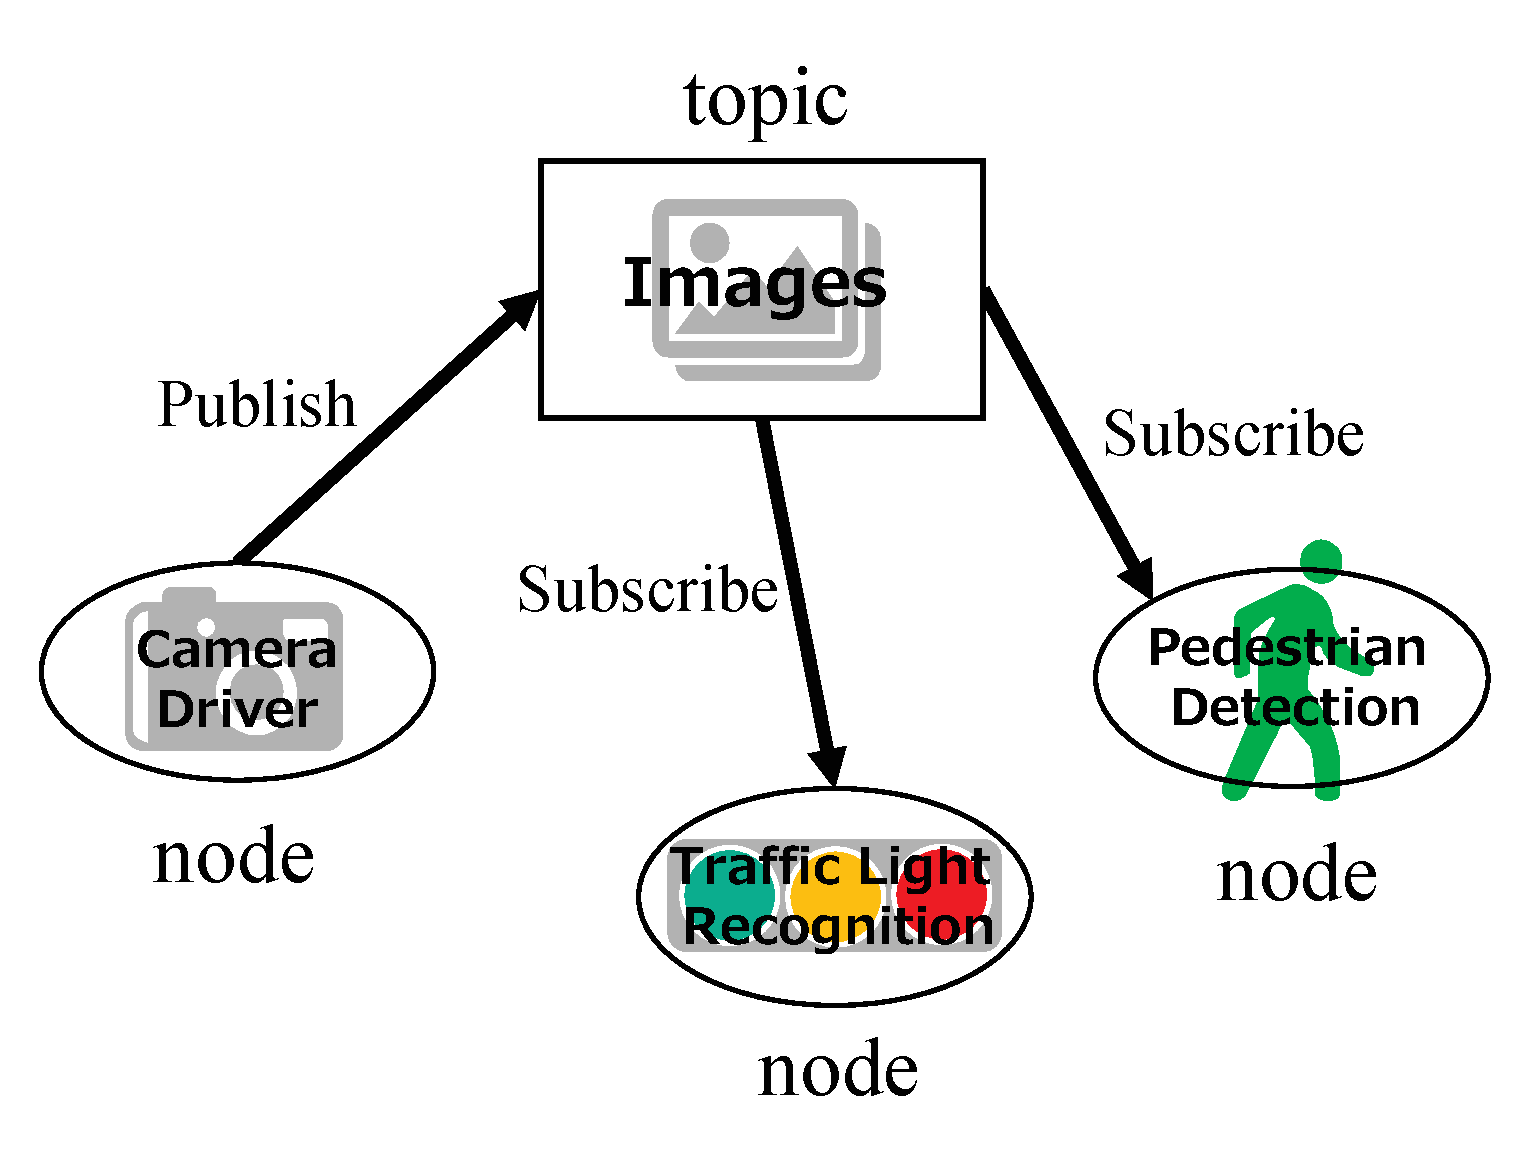
\includegraphics[width=0.8\linewidth]{../figure/ros_pubsub.eps}
  \caption{\label{fig:ros_pubsub}
 The publish/subscribe model in ROS.}
\end{figure*}

